% Author :  Lionel du Peloux
% Contact : lionel.dupeloux@gmail
% Year : 2017
% !TEX encoding = UTF-8 Unicode

\chapter{Elastic rod~: variational approach}
\label{sec:ch_energy}

This chapter should be understood as an extension of the work initiated by \citef{Tayeb2015a} and published by \citef{DuPeloux2015} and \citef{Lefevre2017}.

% #######################################################
\section{Introduction}
% #######################################################

Elastic gridshells are lightweight structures made of interconnected slender beams (see \cref{chp:gridshell}). Modeling the deformation process of such structures is complex as it involves to take account for the geometric non linearities induced by the large displacements and rotations of the grid. More over, the large number of connexions and the coupling between flexion and torsion highly increase the complexity of the analysis.

To facilitate the design process of elastic gridshells, architects and engineers need a dedicated numerical tool that provide a good level of interactivity -- which means that numerical computations must converge within a reasonable time, if not in real time -- and gives deep insights on the geometry and on the mechanical behavior of the grid. This tool must be able to model complex connexions and various types of support conditions to enhance the user experience during the formfinding stage and to improve his ability to explore the space of constructible shapes.

In this chapter, our goal is to develop a beam model suitable for the modeling of grids of interconnected slender beams in order to study the mechanics of elastic gridshells. For such beams, Kirchhoff's theory of rods is considered to be appropriate. We follow recent advances in the field of computer graphics about hair modeling \cite{Bergou2008} to build a reduced degrees of freedom rod model thanks to an appropriate curve-angle representation. This representation is based on a relevant curve framing, namely the Bishop frame presented in \cref{sec:bishop}. The rod will be considered inextensible. Moreover, it will be assumed that cross-sections remain normal to the rod centerline. The internal forces and moments acting on the rod will be deduced from the differentiation of the elastic energy of the beam with respect to the degrees of freedom of the system.

This chapter is devoted to the development of the beam model. The formulation of a discrete element and its implementation in a numerical solver are treated in a dedicated chapter (see \cref{chp:numerical_model}).

\subsection{Overview}
We begin this chapter by presenting Kirchhoff model of rods based on two main hypothesis~: the inextensibility and the Euler-Bernouili assumption (see \cref{sec:kirchhoff_rod}). We introduce a \dofs{6} representation of the rod composed of a centerline and a material frame. Thanks to a convenient reference frame we reduce this formulation to \dofs{4} and adopt a curve-angle description of the rod (see \cref{sec:crvangle}). From there, we formulate a variational problem that will lead to the calculation of the internal forces and moments acting on the rod (see \cref{sec:varpb}). We calculate the gradients of the elastic energy to obtain the internal twisting moment (see \cref{sec:dE_dtheta}) and the internal forces (see \cref{sec:dE_dx}). Finally, we discuss the potential of our model and suggest new possibilities (see \cref{sec:discussVar}).

\subsection{Contributions}
\begin{itemize}
\item We consolidate the mathematical development of the beam model by introducing the Fréchet and Gateaux derivatives in function spaces.
\item We clarify the independence of the the rotational degree of freedom ($\theta$) with respect to  translational degrees of freedom ($\vect{x}$).
\item We factorize the expressions of the internal forces and moments by reusing the quasi-static assumption.
\item We identify the contributions of axial and shear forces, bending and torsion moments in the expressions of internal forces and moments.
\item We prove the equivalence with the shear force obtained from the dynamical equations of Kirchhoff.
\item We suggest that the dynamical Kirchhoff equations should be a more straight forward starting point to build up similar theories.
\end{itemize}

\subsection{Related work}
\citef{Bergou2008} present a discrete treatment of adapted framed curves, parallel transport, and holonomy. Based on this framework they propose a curve-angle representation of the geometric configuration of slender rods. In this representation, the orientation of the material frame is established with respect to the Bishop frame by a single scalar angle. Upon this representation they build a mechanical model for slender elastic rods with anisotropic cross-section and arbitrary rest configuration. In the dynamic the centerline is treated explicitly and material frames are treated as quasistatic. \citef{Bergou2010} improve there previous model for the modeling of viscous threads.

\citef{Nabaei2014} implements the model developed by \cite{Bergou2008} in IPOPT, an interior point optimizer, to solve the static equilibrium of simply connected systems of twisted elastica.

\citef{Tayeb2015a}, \citef{DuPeloux2015} and \citef{Lefevre2017} follow \cite{Bergou2008} to model grids of interconnected slender beams. They implement their model in a dynamic relaxation solver to formfind elastic gridshells. They formulate a special connexion.

\citef{Gregoire2007} use the Cosserat theory of rods to simulate naturally straight hoses (application to wire routing or assembly simulation for the automotive industry). The material frame is parametrized by a global rotation using quaternions. The simulation is treated in a quasi-static manner. The problem is formulated as an energy minimization problem solved with newton, conjugate gradient or steepest descent method. \citef{Theetten2008} formulate a geometrically exact dynamic spline model for the simulation of one dimensional objects. They handle elastic and plastic deformations as fracture. \citef{Bertails2006} model the non linear behavior of hair strands with super-helicies. This work is extended later by \citef{Bertails2012} using super-clothoids. This methods have the advantage to postulate a precise geometric interpolation at each point of the rod. \citef{Spillmann2007} adopt a somehow similar approach. They remark that solving directly the Lagrangian equations of motion by a gradient method is too expensive. Thus, they fall back to a semi-implicit Euler integration scheme.

\citef{Jung2010} provide a deep insight to the discrete mechanics of Cosserat rods, as discrete mechanics is a field of research of growing importance.

\citef{Fuller1978}, \citef{Vauquelin2000}, \citef{deVries2005} and \citef{Berger2009} are worth to read to understand the variation of the parallel transport when deforming a path.

%Quaternions also lack singular points and gimbal lock, contrarily to Euler or Cardan angles.


% #######################################################
\section{Kirchhoff rod}\label{sec:kirchhoff_rod}
Kirchhoff's theory of rods is presented thoroughly in the next chapter (see \cref{chp:kirchhoff}). In this chapter, although the assumptions are not exactly the ones made by  Kirchhoff in his theory, we will stick to this denomination as introduced by \cite{Bergou2008}. In the present theory we will assume that~:
\begin{itemize}
\item the rod is inextensible,
\item cross-sections remain plane,
\item cross-sections remain perpendicular to the centerline,
\item the material deforms elastically.
\end{itemize}

\subsection{Description of the motion}\label{sec:description_motion}
We introduce a curvilinear coordinate system to describe the motion of our Kirchhoff rod, compatible with the model assumptions. It is composed of a parametric space curve, called the \emph{centerline}, equipped with a moving frame, called the \emph{material frame}.

\subsubsection{Deformed configuration}
The actual geometric configuration of the rod is described by its centerline $\vect{x}(s)$ and its cross-sections. The centerline is a space curve parameterized by its arc length, denoted $s$. Cross-sections orientation are followed along the centerline by a material frame $\{\vect{d}_3 (s),\vect{d}_1 (s),\vect{d}_2 (s)\}$ which is an adapted orthonormal moving frame aligned with the principal axes of inertia of the cross-section.

Recall from \cref{sec:amf} that \emph{adapted} means that the material frame is aligned with the tangent vector of the centerline~:
\begin{equation}
	\vect{d}_3 (s)=\vect{x}'(s)=\vect{t}(s)
\end{equation}
Here, the prime symbol denotes the derivation with respect to the arc length parameter $s$. Recall also from \cref{sec:arclength_param} that $\norm{\vect{x}'(s)}=1$ because $\vect{x}$ is parametrized by arc length.

\subsubsection{Stress-free configuration}
Among all the possible geometric configurations of the rod we identify the \emph{stress-free configuration} or \emph{rest configuration}, that is the configuration in which the rod is stress-free under no external forces and moments applied top it (loads, supports, \telp{}). This configuration is crucial as the elastic energy of a rod in a given configuration relies on both its actual and rest configuration.

Hereinafter, the symbols referring to this configuration will be denoted with an overbar (e.g. $\rconf{\vect{x}}(s)$).

\subsection{Inextensibility assumption}
As explained by \citef{Audoly2010}, based on a scaling argument, two cases arise for slender beams~: either the centerline stretches and bending and twisting forces become negligible compared to axial forces~; either the centerline remains inextensible. As we are not interested in the first case -- in which the beam would behave like a cable, mainly in tension -- we will assume that the rod is effectively inextensible.\footnote{For a complete treatment of the question of inextensibility refer to \cref{sec:kirchhoff_motion} in \cref{chp:kirchhoff}.}

Remark that the previous description (see \cref{sec:description_motion}) is only valid for inextensible rods. Indeed, for an inextensible rod the centerline does not stretches and the arc length parameter for the rest configuration is also a valid arc length parameter for any other configuration.\footnote{For a complete treatment of the question of reparametrization refer to \cref{sec:cosserat_motion} in \cref{chp:kirchhoff}.}

The inextensibility hypothesis also implies that any admissible perturbation ($\lambda\vect{h}_x$) of the rod's centerline ($\vect{x}$) is locally orthogonal to the centerline itself. Indeed, at each arc length $s$ an inextensible rod must satisfies~:
\begin{equation}
	\|\vect{x}'\| = \|(\vect{x}+\lambda\vect{h}_x)'\| = 1 \Rightarrow \vect{d}_3 \cdot \vect{h}'_x = -\tfrac{\lambda^2}{2}\|\vect{h}'_x\|^2 = o(\lambda) \simeq 0
	\label{eq:axialstrain}
\end{equation}
It is worth to mention here that this property ($\vect{d}_3 \cdot \vect{h}'_x = 0$) will be used several times in the following sections.

Hereinafter, the length of the rod will be denoted $L$ and the arc length $s$ will vary in $[0,L]$, with no loss of generality.

\subsection{Euler-Bernouilli assumption}
Strains are supposed to remain small so that the cross-sections remain plane and the material frame remains orthonormal and adapted to the centerline during the motion of the rod. In other words the cross-sections undergo rigid body motions.\footnote{For a complete treatment of this point in Kirchhoff's theory refer to \cref{sec:kirchhoff_deform_conf} in \cref{chp:kirchhoff}.}

\subsection{Motion of the material frame}
As a consequence of the Euler-Bernoulli assumption, we can differentiate the conditions of orthonormality of the material frame (see \cref{sec:moving_frame}). This leads to the following system of differential equations governing the evolution of the \emph{material directors} $\{\vect{d}_3 (s),\vect{d}_1 (s),\vect{d}_2 (s)\}$ along the centerline~:
\begin{equation}
	\begin{bmatrix}
		\vect{d}'_3(s) \\
		\vect{d}'_1(s) \\
		\vect{d}'_2(s)
	\end{bmatrix}
	=
	\begin{bmatrix*}[c]
		0 & \phantom{-}\kappa_{2}(s) & -\kappa_{1}(s) \\
		-\kappa_{2}(s) & 0 & \phantom{-}\tau(s) \\
		\phantom{-}\kappa_{1}(s) & -\tau(s) & 0
	\end{bmatrix*}
	\begin{bmatrix}
		\vect{d}_3(s) \\
		\vect{d}_1(s) \\
		\vect{d}_2(s)
	\end{bmatrix}
	\label{eq:mf_motion}
\end{equation}
where $\tau(s)$, $\kappa_{1}(s)$ and $\kappa_{2}(s)$ are the rates of rotation of the material frame with respect to the arc length parameter $s$. These equations can be formulated with the \emph{Darboux vector} of the chosen material frame, which represents the angular velocity vector of the frame along $\vect{x}(s)$~:
\begin{subequations}
	\begin{alignat}{2}
		&\vect{d}'_{i}(s) = \vect{\Omega}_m(s) \times \vect{d}_i(s)
		\\[0.5em]
		&\vect{\Omega}_m(s) = \begin{bmatrix} \tau(s) \\ \kappa_{1}(s) \\ \kappa_{2}(s)
	\end{bmatrix}
	\end{alignat}
\end{subequations}
That means that $\tau(s)$, $\kappa_{1}(s)$ and $\kappa_{2}(s)$ are the components of the angular velocity of the material frame around its axes $\vect{d}_3 (s)$, $\vect{d}_1 (s)$ and $\vect{d}_2 (s)$ when it travels along the centerline at unit speed.\footnote{See \cref{fig:geo_interpretation} in \cref{sec:moving_frame} for a geometric interpretation of these rates of rotation.}

Recall from \cref{sec:curvature} how the (geometric) curvature ($\kappa$) of a spatial curve parametrized by arc length is related to the Frenet frame $\{\vect{t}(s),\vect{n}(s),\vect{b}(s)\}$ by ~:
\begin{subequations}
	\begin{alignat}{2}
		&\vect{t}'(s) = \vect{x}''(s) = \kappa(s) \cdot \vect{n}(s)
		\\
		&\kappa(s) = \norm{\vect{t}'(s)} = \norm{\vect{x}''(s)}
		\\
		&\vect{b}(s) = \vect{t}(s) \times \vect{n}(s)
	\end{alignat}
\end{subequations}
To describe the osculating plane in which lies the bending part of the deformation we rely on the \emph{curvature binormal} introduced previously in \cref{eq:kb}. We recall from \cref{eq:kb,eq:kb_components} that~:
\begin{equation}
	\vect{\kappa b}(s) = \kappa(s) \cdot \vect{b}(s) = \vect{t}(s)\times\vect{t}'(s) = \kappa_1(s)\vect{d}_1(s) + \kappa_2(s)\vect{d}_2(s)
\end{equation}
The curvature binormal is the vector of direction $\vect{b}(s)$ and norm $\kappa(s)$, and at each point of arc length $s$ the osculating plane is normal to $\vect{\kappa b}(s)$. Finally, recall from \cref{eq:angular_velocity} that, as the material frame is adapted to the centerline, the following equation holds~:
 \begin{equation}
	\vect{\Omega}_m(s) = \vect{\kappa b}(s)  + \tau(s) \vect{t}(s)
\end{equation}

\subsection{Material curvatures and twist}
Kirchhoff's theory assigns a physical meaning to the components of $\vect{\Omega}_m(s)$~:
\begin{itemize}
\item $\kappa_1(s)$ and $\kappa_2(s)$ are called the \emph{material curvatures} and represent the rod's flexion in the principal planes, respectively normal to $\vect{d}_1(s)$ and $\vect{d}_2(s)$ (see \cref{fig:curve_angle_a})~;
\item $\tau(s)$ is called the \emph{material twist} and represents the cross-sections rate of rotation around $\vect{d}_3(s)$ (see \cref{fig:curve_angle_b}).
\end{itemize}
These scalar functions are directly related to the components of the strain tensor as defined in Kirchhoff's theory.\footnote{For a complete treatment of the definition of  strain in Kirchhoff's theory refer to \cref{sec:kirchhoff_strains} in \cref{chp:kirchhoff} or \citef{Dill1992}}

Note that In the literature these quantities are sometimes called \emph{strain rates} (\citef{Antman2005}) or moment strains (\citef{Reissner1973}). However, this depart from the most common definition in which the strain is a dimensionless quantity~: \blockcquote[p.~19]{Audoly2010}{The theory of elasticity deals with solids that, in the presence of mechanical stress, depart from their \textquote{natural} configuration \belp{}. The strain provides a geometrical characterization of deformation~: it measures by how much the solid departs from its natural configuration.}.

\subsection{Material constitutive equations}
The twisting moment ($Q$) and the components of the bending moment ($M_1$, $M_2$) are determined through the usual material constitutive equations~:
\begin{subequations}
	\begin{alignat}{2}
		Q = GJ (\tau_1 - \rconf{\tau_1}) \label{eq:Q}\\
		M_1 = EI_1 (\kappa_1 - \rconf{\kappa_1}) \label{eq:M1}\\
		M_2 = EI_2 (\kappa_2 - \rconf{\kappa_2}) \label{eq:M2}
	\end{alignat}
\end{subequations}
We also introduce the vector of internal moments and its as~:
\begin{subequations}
	\begin{alignat}{2}
		&\vect{M} &&= Q\vect{d}_3 + M_1\vect{d}_1 + M_2\vect{d}_2 \\
		&\vect{M}^{\perp} &&= M_1\vect{d}_1 + M_2\vect{d}_2 
	\end{alignat}	
\label{eq:vM}
\end{subequations}

\subsection{Elastic energy}
Kirchhoff's theory assigns an elastic energy to beams according to their strain~\cite{Audoly2010}. In this theory, a beam is supposed to be inextensible. Thus the elastic energy ($\mathcal{E}$) only accounts for bending and torsion and behaviors and is given by~:
\begin{equation}
	\mathcal{E} =
	\tfrac{1}{2} \int_{0}^{L}EI_1(\kappa_1-\rconf{\kappa}_1)^2 + EI_2(\kappa_2-\rconf{\kappa}_2)^2 ds
	+ \tfrac{1}{2} \int_{0}^{L} GJ(\tau -{\rconf{\tau}})^2 ds
	\label{eq:energy_el}
\end{equation}
Here, $\rconf{\kappa}_1$, $\rconf{\kappa}_2$ and $\rconf{\tau}$  denote the \emph{natural} material curvatures and material twist of the rod in its rest configuration. $E$ and $G$ are the elastic and shear modulus of the material. $I_1$ and $I_2$ are the moments of inertia of the cross-section. $J$ is the torsion constant of the cross-section.

\subsubsection{Initially straight isotropic rod~: a special case}
From this energy formulation an interesting an well-known result on elastic rods can be retrieved.\footnote{For instance, this result is cited by \citef{Adriaenssens1999}.}. This results stipulates that torsion is uniform in a rod with isotropic cross-section and naturally straight.

Indeed, by definition for a rod with isotropic cross-section~: $EI_1 = EI_2 = EI$. If in addition the rod is straight in its rest configuration~: $\rconf{\kappa}_1 = \rconf{\kappa}_2 = \rconf{\tau} = 0$. The bending energy becomes~: $\mathcal{E}_{b} = EI_1\;\kappa_1^2 + EI_2\;\kappa_2^2 = EI(\kappa_1^2 + \kappa_2^2) = EI\kappa^2$. Consequently, the elastic energy of the rod is composed of two independent terms~: $\mathcal{E}_{b}[\vect{x}]$ and $\mathcal{E}_{r}[\theta]$. The coupling between bending and twisting disappears and the global minimum of elastic energy is reached when minimizing separately bending an twisting energies. This meansthat the geometry of the rod at static equilibrium ($\vect{x}$) is the one that minimized $\mathcal{E}_{b}[\vect{x}]$. And the minimum of $\mathcal{E}_{t}[\theta]$ is obviously achieved for a uniform twist ($\tau = cst$) along the centerline, only prescribed by the boundary conditions at the extremities of the rod (least-squares minimization).

In that particular case, the geometry of the centerline is not influenced by the amount of uniform twist (hence torsion) present in the rod.

\section{Curve-angle representation}\label{sec:crvangle}

In the previous paragraph we have shown how the elastic energy of a rod can be computed with respect to the position of its centerline and the orientation of its cross-sections. This representation can be naturally described with six degrees of freedom (\dofs{6})~: \footnote{This is the usual choice in which the orientation of the material frame is parametrized by a rotation matrix, or equivalently a quaternion.}
\begin{itemize}
\item \dofs{3} for the position of the centerline,
\item and \dofs{3} for the orientation of the cross-sections.
\end{itemize}

Following~\citef{Bergou2008} we introduce a reduced coordinate formulation of the rod that accounts for only \dofs{4}~:
\begin{itemize}
\item \dofs{3} for the position of the centerline,
\item and only \dofs{1} for the orientation of the cross-sections.
\end{itemize}
\begin{figure}[t]
%	\begin{fullpage}
     		\centering
		\subfloat[][bending strains]{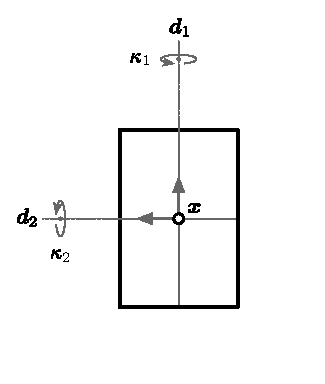
\includegraphics{curve_angle_a.pdf}\label{fig:curve_angle_a}}
		\hspace{2.5cm}
		\subfloat[][angular deviation]{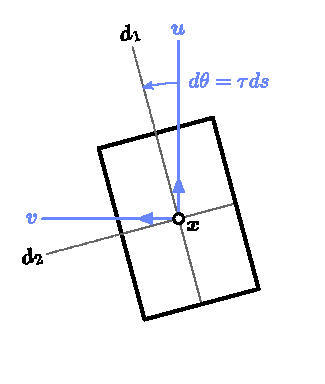
\includegraphics{curve_angle_b.pdf}\label{fig:curve_angle_b}} \\
		\vspace{10pt}
		\captionof{figure}[Curve-angle representation of the rod]{Curve-angle representation of the rod. The orientation of the material frame is established from the reference frame by the deviation angle $\theta(s)$.}
		\label{fig:curve_angle}    
%	\end{fullpage}
\end{figure}

\subsection{Definition of the representation}
This reduction of the number of \dofs{} relies on the choice of a suitable reference frame, namely a Bishop (or zero-twisting) frame denoted $\{\vect{t}(s),\vect{u}(s),\vect{v}(s)\}$. Recall from \cref{sec:bishop} in \cref{chp:curve} that this reference frame is adapted to the centerline and exhibits a null angular velocity around the centerline's tangent vector (see \cref{eq:null_velocity}), which means~:
\begin{equation}
	\vect{u}(s)\cdot\vect{v}'(s) = \vect{u'}(s)\cdot\vect{v}(s)=0
\end{equation}
The Bishop frame only depends on $\vect{x}$, the geometry of the centerline, and the choice of an initial condition. This reference frame is obtained all along the curve by propagating a given initial frame -- usually chosen at $s=0$ -- with the parallel transport operator (see \cref{sec:paralleltransport}). By construction, this reference frame evolves along the curve with the following angular velocity~:
\begin{subequations}\label{eq:bishop_motion}
	\begin{alignat}{2}
	&\vect{\Omega}_b(s)&&=\vect{\kappa b}=\vect{t}\times\vect{t}'=\vect{x}'\times\vect{x}'' \label{eq:kb2}\\
	&\vect{t}'(s)&&=\vect{\kappa b} \times \vect{t} \\
	&\vect{u}'(s)&&=\vect{\kappa b} \times \vect{u} \\
	&\vect{v}'(s)&&=\vect{\kappa b} \times \vect{v}
	\end{alignat}
\end{subequations}
Remark that $\vect{\Omega}_b(s)$ only depends on the centerline and is well defined even when the curvature vanishes, unlike the Frenet frame. In that case the parallel transport operator becomes the rotation of null angle, which is still a valid transformation.

Hence, the orientation of the cross-sections, that is the material frame $\{\vect{d}_3 (s),\vect{d}_1 (s),\vect{d}_2 (s)\}$, can be tracked only by the measure of a single angle $\theta(s)$ from this reference frame denoted $\{\vect{d}_3(s),\vect{u}(s),\vect{v}(s)\}$~:
\begin{equation}
	\begin{bmatrix}
		\vect{d}_1(s)\\
		\vect{d}_2(s)\\
	\end{bmatrix} =
		\begin{bmatrix}
		\cos{\theta(s)} & \sin{\theta(s)}\\
		-\sin{\theta(s)} & \cos{\theta(s)}\\
	\end{bmatrix}
	\begin{bmatrix}
		\vect{u}(s)\\
		\vect{v}(s)\\
	\end{bmatrix}
	\label{eq:crvangle_matrix}
\end{equation}
Note that the choice of an initial condition for the definition of the Bishop frame is not a matter of concern as only the derivative of $\theta$ appears in the elastic energy (see \cref{eq:energy_el}). Thus, we are free to choose this condition in the most convenient way.

\subsection{Measurement of the material twist}
With this \dofs{4} representation, the material twist is directly expressed in terms of the derivative of $\theta$. Indeed, from \cref{eq:crvangle_matrix,eq:bishop_motion} we obtain~:
\begin{equation}
	\begin{aligned}
		\vect{d}'_1 
			&= (\cos{\theta} \vect{u} + \sin{\theta}\vect{v})' \\
			& = (-\sin{\theta} \vect{u} + \cos{\theta}\vect{v})\cdot \theta' +  \cos{\theta} \vect{u}' + \sin{\theta}\vect{v}' \\
			& = \theta' \vect{d}_2 + \cos{\theta}\; (\vect{\kappa b} \times \vect{u}) + \sin{\theta}\; (\vect{\kappa b} \times \vect{v})\\
			& = \theta' \vect{d}_2 + \vect{\kappa b} \times \vect{d}_1\\
	\end{aligned}
\end{equation}
Finally, using the definition of $\tau$ from \cref{eq:mf_motion} and the fact that $\vect{\kappa b}$ is perpendicular to $\vect{d}_3$ we can deduce that $\tau=\theta'$~:
\begin{equation}
	\tau = \vect{d}'_1 \cdot \vect{d}_2 = (\theta'\vect{d}_2 + \vect{\kappa b}\times\vect{d}_1)\cdot \vect{d}_2 = \theta' + \vect{d}_3\cdot\vect{\kappa b} = \theta'
\label{eq:thetatau}
\end{equation}
Here, the benefits of the curve-angle representation are revealed as the material twist is now simply given by the rate of $\theta$ with respect to the arc length parameter $s$. Everything happens as if the Bishop would enable a directe measurement of the mechanical torsion, getting ride of the intrinsic geometric torsion of the centerline itself (aka the torsion of Frenet).
\subsection{Vector of material curvatures}
We introduce the vector of material curvatures ($\vect{\omega}$) as the 2-dimensional vector of components $\kappa_1$ and $\kappa_2$~:
\begin{equation}
	\vect{\omega} =
	\begin{bmatrix*}[r]
		\kappa_1\\
		\kappa_2\\
	\end{bmatrix*} =
	\begin{bmatrix}
		\vect{\kappa b}\cdot\vect{d}_1\\
		\vect{\kappa b}\cdot\vect{d}_2\\
	\end{bmatrix} =
	\begin{bmatrix*}[r]
		-\vect{x}''\cdot\vect{d}_2\\
		\vect{x}''\cdot\vect{d}_1\\
	\end{bmatrix*}
\end{equation}

\section{Definition of the variational problem}\label{sec:varpb}
We now have all the ingredients to build the variational problem that will lead us to the determination of the internal forces ($\vect{f}$) and the internal twisting moment ($\vect{m}$) acting on the centerline. Indeed, the quasi-static out-of-balance internal forces and twisting moment acting on the beam are calculated by differentiating the elastic energy of the system with respect to the 4 \dofs{} of the system, namely $\vect{x}$ and $\theta$.

\subsection{Calculus of variations}
Differentiating $\mathcal{E}$ with respect to $\vect{x}$ will yield the linear resultant of the internal forces ($\vect{f}$, see \cref{sec:dE_dtheta}), while differentiating $\mathcal{E}$ with respect to $\theta$ will yield the linear resultant of the internal twisting moment ($\vect{m}$, see \cref{sec:dE_dx}). Main results for the calculus of variations are reminded in \cref{chp:variation}.

These forces and moments will be used later in a damped explicit dynamic procedure to solve the equilibrium of the system. However, they are nothing but the gradient of the elastic energy and any other variational method can be employed to find a geometric configuration that minimize the elastic energy, that is a configuration in which the rod is at static equilibrium (our ultime goal).

Introducing $\vect{\omega}$ and $\theta$, the elastic energy defined in \cref{eq:energy_el} can be rewritten in the form~:
\begin{equation}
		\mathcal{E} = \mathcal{E}_{b} + \mathcal{E}_{t} =
		\tfrac{1}{2} \int_{0}^{L} (\vect{\omega}-\rconf{\vect{\omega}})^T B (\vect{\omega}-\rconf{\vect{\omega}}) ds
		+ \tfrac{1}{2} \int_{0}^{L} \beta(\theta' -{\rconf{\theta}'})^2 ds
\label{eq:E2}
\end{equation}
where $B$ is the bending stiffness matrix given in material frame coordinate system and $\beta$ is the torsional stiffness given by~:
\begin{equation}
	B(s) = \begin{bmatrix}
			EI_1(s)	&	0\\
			0	&	EI_2(s)\\
		\end{bmatrix}
	\quad,\quad
	\beta(s) = (GJ)(s)
\end{equation}
The matrix notation introduced in \cref{eq:E2} will enable more compact forms for equations. It will be used through out this chapter. Remark who the scalar product of vectors is treated as matrix multiplication with a row and column vector.

The internal shear forces and the internal twisting moment are then given by~:
\begin{subequations}
	\begin{alignat}{2}
		&\vect{f} &&= - \frac{\partial \mathcal{E}}{\partial \vect{x}} [\vect{x}, \theta] \\[0.5em]
		&\vect{m} &&= - \frac{\partial \mathcal{E}}{\partial \theta}[\vect{x}, \theta] \cdot \vect{d}_3
	\end{alignat}
\end{subequations}
It is importante to notice that as the rod is supposed to be inextensible, the elastic energy does not include any term to characterized the axial strain. This assumption will have to be treated as a constraint when solving the variational problem. For instance, \citef{Bergou2008} choose to enforce inextensibility at each time step with a reprojection algorithm while \citef{Lefevre2017} choose to enforce this constraint thanks to a penalty energy. Hence, $\vect{f}$ will give only the internal shear forces acting on the centerline.\footnote{This is somehow equivalent to what is remarked by Dill~: \blockcquote[]{Dill1992}{The resultant shears $F_1$ and $F_2$ are not determined by the constitutive equations. They are reactive parameters in the equations of balance of momentum as they are in the elementary beam theory.}.}

\subsection{Prerequisite for the computation of energy gradients}
To compute the energy gradients with respect to the degrees of freedom of the rod it is primordial to understand how these \dofs{} are chained (see \cref{fig:dofs})~:
\begin{figure}[h]
     		\centering
     		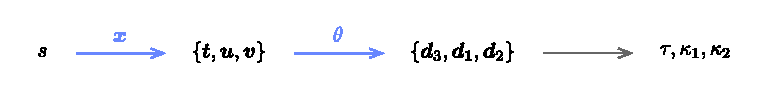
\includegraphics{degrees_of_freedom.pdf}
%		\vspace{10pt}
		\captionof{figure}[Succession of the degrees of freedom]{Succession of the degrees of freedom.}
%		\vspace{10pt}
		\label{fig:dofs}    
\end{figure}
\begin{itemize}
\item 
$\vect{x}$ leads to the determination of the curvature binormal ($\vect{\kappa b}$) and to the determination of the reference Bishop frame $\{\vect{t},\vect{u},\vect{v}\}$.
\item 
$\theta$ leads to the determination of the material frame $\{\vect{t},\vect{d}_1,\vect{d}_1\}$ from the reference frame $\{\vect{t},\vect{u},\vect{v}\}$.
\item 
$\kappa_1$ and $\kappa_2$ are the projections of $\vect{\kappa b}$ on $\vect{d}_1$ and $\vect{d}_2$. This means that $\vect{\omega}$ depends on $\vect{x}$ through the determination of $\vect{\kappa b}$ and the determination of $\{\vect{t},\vect{u},\vect{v}\}$ ; and depends on $\theta$ through the determination of $\{\vect{d}_1, \vect{d}_2\}$ from $\{\vect{u}, \vect{v}\}$.
\item 
$\tau$ only depends on $\theta$ and is thus independent of $\vect{x}$.
\end{itemize}


\subsection{Coupling between bending and torsion}
Remark that the twisting energy ($\mathcal{E}_{t}$) only depends on $\theta$ and is independent regarding $\vect{x}$ while the bending energy ($\mathcal{E}_{b}$) depends on both $\theta$ and $\vect{x}$ variables (remind that $\kappa_1$ and $\kappa_2$ are the projections of $\vect{\kappa b}$ over $\vect{d}_1$ over $\vect{d}_2$). Thus, a coupling between bending and twisting appears and the minimum of the whole elastic energy is not necessarily reached for concomitant minimums of bending and twisting energies.

\subsection{Quasistatic assumption}
Following~\citef{Bergou2008}, it is relevant to assume that the propagation of twist waves is instantaneous compared to the propagation of bending waves because for slender rods the axial stiffness is usually an order of magnitude higher than the bending stiffness. This means that the distributed internal forces ($\vect{f}$) and the  distributed internal moment of torsion ($\vect{m}$) act on two different timescales in the rod dynamic.

Thus, on the timescale of action of the internal forces on the center line, driving the bending waves, the twist waves propagate instantaneously, so that~:
\begin{equation}
	\frac{\partial \mathcal{E}}{\partial\theta}[\vect{x}, \theta]=0
\label{eq:quasistat_hyp}
\end{equation}
for the computation of $\vect{f}$.

This assumption is not mandatory -- for instance it is not made by \citef{Nabaei2014} -- but was found to lead to simpler and faster computations.

\section{Energy gradient with respect to $\theta$~: twisting moment}\label{sec:dE_dtheta}

For the calculus of variations, the reader is invited to refer to \cref{chp:variation} where the notations employed through out this section are defined and where main results are reminded. 

\subsection{Derivative of material directors with respect to $\theta$}
Recalling that $\theta$ and $\vect{x}$ are independant variables and that the Bishop frame $\{\vect{u},\vect{v}\}$ only depends on $\vect{x}$, the decomposition of the material frame directors $\{\vect{d}_1,\vect{d}_2\}$ on the Bishop frame leads directly to the following expression for the derivative of the material directors~:
\begin{subequations}
\begin{alignat}{1}
	\pdiffof{\theta}{\vect{d}_1}{s}{h_\theta}
	&= \frac{d}{d\lambda} \vect{d}_1[\theta + \lambda h_\theta]\Bigr|_{\lambda = 0} \\ \nonumber
	&= \left(-\sin{\theta}\;\vect{u} + \cos{\theta}\;\vect{v}\right) \cdot h_\theta  \\ \nonumber
	&= \vect{d}_2\cdot h_\theta
	\\[1em]
	\pdiffof{\theta}{\vect{d}_2}{s}{h_\theta}
	&= \frac{d}{d\lambda} \vect{d}_2[\theta + \lambda h_\theta]\Bigr|_{\lambda = 0}  \\ \nonumber 
	&= \left(-\cos{\theta}\;\vect{u} - \sin{\theta}\;\vect{v}\right) \cdot h_\theta   \\ \nonumber
	&= -\vect{d}_1\cdot h_\theta
\end{alignat}
\end{subequations}
where $\fonction{h_\theta}{s}{h_\theta(s)}$ denotes a small perturbation of $\theta$ and $\pdiff{\theta}{\vect{d}_i}{s}$ denotes the derivative of $\vect{d}_i$ at $s$ with respect to $\theta$. When it is appropriate, brackets are employed to signal important functional dependencies, while parenthesis will denote the dependence with respect to the arc length parameter $s$.

\subsection{Derivative of the material curvatures vector with respect to $\theta$}
Regarding the definition of the material curvatures vector and the derivative of material directors with respect to $\theta$, it follows immediately that~:
\begin{equation}
\begin{aligned}
	\pdiffof{\theta}{\vect{\omega}}{s}{h_\theta}
	&= \frac{d}{d\lambda} \vect{\omega}[\theta + \lambda h_\theta]\Bigr|_{\lambda = 0} 
	\\[0.5em]
	&= \begin{bmatrix*}[r]
		\vect{\kappa b}\cdot\vect{d}_2\\
		-\vect{\kappa b}\cdot\vect{d}_1\\
	\end{bmatrix*}\cdot h_\theta \\
	&= - \mat{J}\vect{\omega}\cdot h_\theta
\end{aligned}
\label{eq:DthetaW}
\end{equation}
where $\mat{J}$ is the matrix that acts on two dimensional vectors by counter-clockwise rotation of angle $\frac{\pi}{2}$~:
\begin{equation}
	\mat{J} = \begin{bmatrix*}[r]
			0	&	-1\\
			1	&	0\\
		\end{bmatrix*}
\end{equation}

\subsection{Computation of the twisting moment}

The distributed moment of torsion is given by the functional derivative of the elastic energy with respect to $\theta$, which can be decomposed into~:
\begin{equation}
	\begin{aligned}
	\scalar{-m(s)}{h_\theta} 
	&= \pdiffof{\theta}{\mathcal{E}}{s}{h_\theta} \\
	&= \pdiffof{\theta}{\mathcal{E}_b}{s}{h_\theta} + \pdiffof{\theta}{\mathcal{E}_t}{s}{h_\theta}
	\end{aligned}
\label{eq:mintdef}
\end{equation}

\subsubsection{Derivative of the torsion energy with respect to $\theta$}
We calculate the partial derivative of the twisting elastic energy with respect to $\theta$ as~:
\begin{equation}
	\begin{aligned}
	\pdiffof{\theta}{\mathcal{E}_t[\theta]}{s}{h_\theta}
		&= \frac{d}{d\lambda} \mathcal{E}_t[\theta + \lambda h_\theta]\Bigr|_{\lambda = 0} \\
		&= \frac{d}{d\lambda}\left( \tfrac{1}{2} \int_{0}^{L} \beta\left((\theta + \lambda h_\theta)' -{\rconf{\theta}'}\right)^2 \;dt \right)\Bigr|_{\lambda = 0} \\
		&= \int_{0}^{L} \beta(\theta' -{\rconf{\theta}'}) \cdot h_\theta' \;dt \\
		&= \left[\beta(\theta' -{\rconf{\theta}'}) \cdot h_\theta\right]_0^L - \int_{0}^{L} \left(\beta(\theta' -{\rconf{\theta}'})\right)' \cdot h_\theta \;dt \\
		&= \int_{0}^{L} \left(\beta(\theta' -{\rconf{\theta}'})(\delta_L-\delta_0) - \left(\beta(\theta' -{\rconf{\theta}'})\right)'\right) \cdot h_\theta \;dt \\
	\end{aligned}
\label{eq:dEtdtheta}
\end{equation}
where $\delta_L$ and $\delta_0$ are the Dirac distributions centered respectively on $s=L$ and $s=°$.
\subsubsection{Derivative of the bending energy with respect to $\theta$}
 
To compute the partial derivative of $\mathcal{E}_b$ with respect to $\theta$ we first calculate the derivative of $\mathcal{E}_b$ with respect to $\vect{\omega}$~:
\begin{equation}
	\begin{aligned}
	\pdiffof{\omega}{\mathcal{E}_b[\vect{\omega}]}{s}{\vect{h}_\omega}
		&= \frac{d}{d\lambda} \mathcal{E}_b[\vect{\omega} + \lambda \vect{h}_\omega]\Bigr|_{\lambda = 0} \\
		&= \frac{d}{d\lambda}\left( \tfrac{1}{2} \int_{0}^{L} \left(\left(\vect{\omega} + \lambda \vect{h}_\omega\right)-\rconf{\vect{\omega}}\right)^T \mat{B} \left(\left(\vect{\omega} + \lambda \vect{h}_\omega\right)-\rconf{\vect{\omega}}\right) \;dt \right)\Bigr|_{\lambda = 0} \\
		&= \int_{0}^{L} \left(\vect{\omega} - \rconf{\vect{\omega}}\right)^T \mat{B} \cdot \vect{h}_\omega \;dt \\
	\end{aligned}
	\label{eq:DwEtheta}
\end{equation}
where $\fonction{\vect{h}_\omega}{s}{\vect{h}_\omega(s)}$ denotes a small perturbation of $\vect{\omega}$. Then, we calculate the derivative of $\mathcal{E}_b$ with respect to $\theta$ from the chain rule and with \cref{eq:DthetaW,eq:DwEtheta}~:
\begin{equation}
	\begin{aligned}
	\pdiffof{\theta}{\mathcal{E}_b[\vect{\omega}[\theta]]}{s}{h_\theta} &=
	\pdiffof{\omega}{\mathcal{E}_b[\vect{\omega}]}{s}{(\pdiffof{\theta}{\vect{\omega}[\theta]}{s}{h_\theta})} \\
	&= - \int_{0}^{L} (\vect{\omega} - \rconf{\vect{\omega}})^T \mat{B} \mat{J}\vect{\omega}\cdot h_\theta \;dt
	\end{aligned}
\label{eq:dEbdtheta}
\end{equation}

\subsubsection{Twisting moment}
The gradient of the elastic energy with respect to $\theta$ is obtained from \cref{eq:mintdef} with \cref{eq:dEbdtheta,eq:dEtdtheta}~:
\begin{equation}
	\begin{aligned}
		\scalar{-m(s)}{h_\theta}
		&= \pdiffof{\theta}{\mathcal{E}_b[\vect{\omega}[\theta]]}{s}{h_\theta} + \pdiffof{\theta}{\mathcal{E}_t[\theta]}{s}{h_\theta} \\
		&= \int_{0}^{L} \left(\left(\beta(\theta' -{\rconf{\theta}'})(\delta_L-\delta_0) - \left(\beta(\theta' -{\rconf{\theta}'})\right)'\right) - (\vect{\omega} - \rconf{\vect{\omega}})^T \mat{B} \mat{J}\vect{\omega}\right) \cdot h_\theta \;dt
	\end{aligned}
\end{equation}
Finally, we can conclude on the expression of the distributed internal twisting moment~:
\begin{equation}
	m(s) = - \left(\beta(\theta' -{\rconf{\theta}'})(\delta_L-\delta_0) - \left(\beta\left(\theta' -{\rconf{\theta}'}\right)\right)'\right)(s) + \left((\vect{\omega} - \rconf{\vect{\omega}})^T \mat{B} \mat{J}\vect{\omega}\right)(s)
\end{equation}
Remark with \cref{eq:thetatau,eq:Q}, respectively with \cref{eq:M1,eq:M2}, that~:
\begin{subequations}
	\begin{alignat}{2}
		&\beta\left(\theta' -{\rconf{\theta}'}\right) = Q \label{eq:Q2}\\
		&(\vect{\omega} - \rconf{\vect{\omega}})^T \mat{B} \mat{J}\vect{\omega} = \kappa_1 M_2 - \kappa_2 M_1
	\end{alignat}
\end{subequations}
Hence, the quasi-static distributed internal twisting moment acting on the centerline is given for all $s$ in $]0,L[$ by~:
\begin{equation}
	m(s) = Q'(s) +  \kappa_1(s) M_2(s) - \kappa_2(s) M_1(s)
\label{eq:mint}
\end{equation}


\subsubsection{Quasistatic hypothesis}
The quasistatic assumption (see \cref{eq:quasistat_hyp}) stipulates that the gradient of the elastic energy with respect to $\theta$ can be considered null ($\pdiff{\theta}{\mathcal{E}}{s} = 0$) for the calculation of the internal forces, which implies that for all $s$ in $[0,L]$~:
\begin{equation}
	\left(\left(\beta(\theta' -{\rconf{\theta}'})\right)' + (\vect{\omega} - \rconf{\vect{\omega}})^T \mat{B} \mat{J}\vect{\omega}\right)(s) = 0
\label{eq:quasistat}
\end{equation}
or equivalently~:
\begin{equation}
	Q'(s) +  \kappa_1(s) M_2(s) - \kappa_2(s) M_1(s) = 0
\label{eq:quasistat}
\end{equation}


\section{Energy gradient with respect to $x$~: internal forces}\label{sec:dE_dx}

For the calculus of variations, the reader is invited to refer to \cref{chp:variation} where the notations employed through out this section are defined and where main results are reminded. 

\subsection{Derivative of material directors with respect to $x$}
A variation of the centerline $\vect{x}$ by $\vect{\epsilon} = \lambda \vect{h}_x$ would cause a variation of the Bishop frame because parallel transport depends on the centerline itself. As far as $\vect{x}$ and $\theta$ are independent variables, this leads necessarily to a variation of the material frame. Let us denote~:
\begin{itemize}
\item
$F = \{\vect{t}, \vect{u},\vect{v}\}$~: the Bishop frame in the reference configuration ;
\item
 $F_\epsilon = \{\vect{t}_\epsilon, \vect{u}_\epsilon,\vect{v}_\epsilon\}$~: the Bishop frame in the deformed configuration ;
 \item
$\tilde{F}_\epsilon = \{\vect{t}, \vect{\tilde{u}}_\epsilon,\vect{\tilde{v}}_\epsilon\}$~: the frame obtained by parallel transporting $F_\epsilon$ back on $F$.
\end{itemize}
\begin{figure}[p]
\begin{fullpage}
\centering
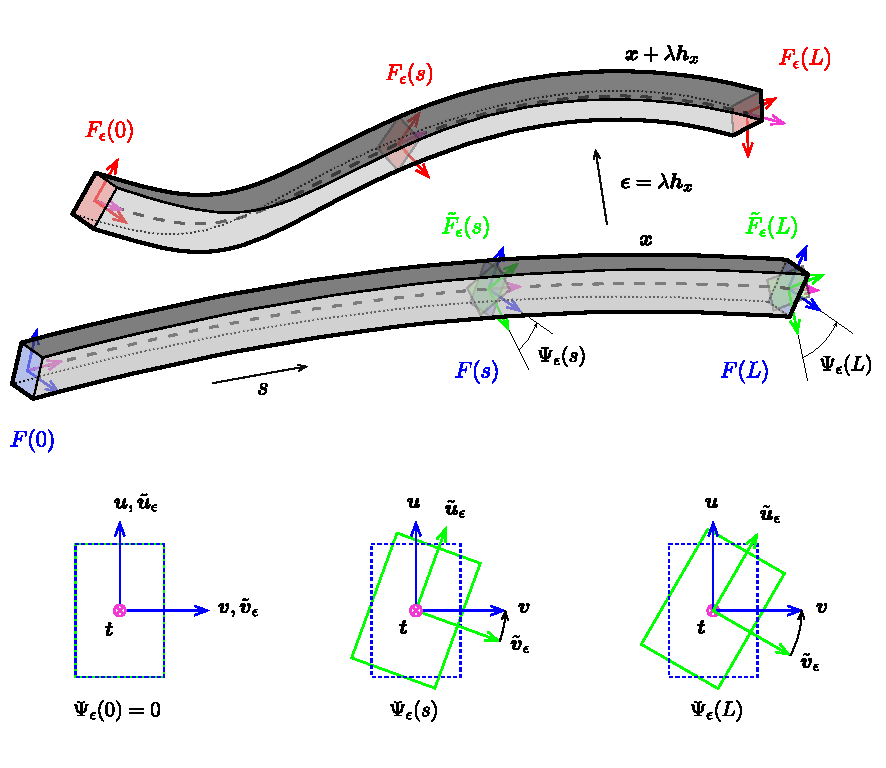
\includegraphics[width=\linewidth]{writhe.pdf}
\captionof{figure}[Variation of the Bishop frame for a perturbation of the centerline]{Variation of the Bishop frame for a perturbation of the centerline.}
\label{fig:varbishop}
\end{fullpage}
\end{figure}
From \cref{fig:varbishop} we start with an (arbitrary) initial reference frame defined in the rest configuration and denoted $F(0)$, positioned at arc length parameter $s=0$~:
\begin{itemize}
\item 
Firstly, the intial frame $F(0)$ is parallel transported along the centerline of the rest configuration into the frame $F(s)$ at arc length parameter $s$ (see \cref{fig:varbishop}).
\item
Secondly the initial frame $F(0)$ is parallel transported at the starting point of the centerline of the deformed configuration into the frame $F_{\epsilon}(0)$. The frame $F_{\epsilon}(0)$ is then parallel transported along the centerline of the deformed configuration into the frame $F_{\epsilon}(s)$ at arc length parameter $s$. Finally, $F_{\epsilon}(s)$ is parallel transported back onto the frame $F(s)$ of the reference configuration. This frame is denoted $\tilde{F}_\epsilon(s)$ (see \cref{fig:varbishop}).
\end{itemize}
The two frames $F(s)$ and $\tilde{F}_\epsilon(s)$ are not aligned as a variation of the centerline has caused a variation of the bishop frame. We call $\Psi_\epsilon(s)$ the amount of rotation around $\vect{t}(s)$ needed to realign $\tilde{F}_\epsilon(s)$ onto $F(s)$ (see \cref{fig:varbishop} where $\Psi_\epsilon(s) < 0$). $\Psi_\epsilon(s)$ characterizes precisely the variation of the parallel transport operator with respect to a perturbation of the centerline.

The sequence of transformations described previously and illustrated in \cref{fig:varbishop} can be decomposed into only two rotations that contribute to $\Psi_\epsilon(s)$~:
\begin{itemize}
\item
$F_\epsilon \rightarrow \tilde{F}_\epsilon$~: parallel transporting $F_\epsilon$ from $\vect{t}_\epsilon$ to $\vect{t}$.
This is equivalent to a rotation around $\vect{b} = \vect{t}_\epsilon \times \vect{t}$ by an angle $\alpha_\epsilon$. This rotation is described in \cref{fig:rot_a}.
\item
$\tilde{F}_\epsilon \rightarrow F$~: aligning $\tilde{F}_\epsilon$ over $F$. This is equivalent to a rotation around $\vect{t}$ by an angle $\Psi_\epsilon$. This rotation is described in \cref{fig:rot_b}.
\end{itemize}
Firstly, let's decompose $\{\vect{t}_\epsilon, \vect{u}_\epsilon,\vect{v}_\epsilon\}$ on the basis $\{\vect{t}, \vect{\tilde{u}}_\epsilon,\vect{\tilde{v}}_\epsilon\}$. Note that $\tilde{F}_\epsilon$ is expressed by rotating $\tilde{F}_\epsilon$ by an angle $\Psi_\epsilon[\vect{x}](s)$ around $\vect{t}$ because $\tilde{F}_\epsilon$ is obtained by parallel transporting $F_\epsilon$ from $\vect{t}_\epsilon$ to $\vect{t}$.



\subsubsection{Calculation of $\Psi_\epsilon$}

\begin{figure}[p]
\centering
	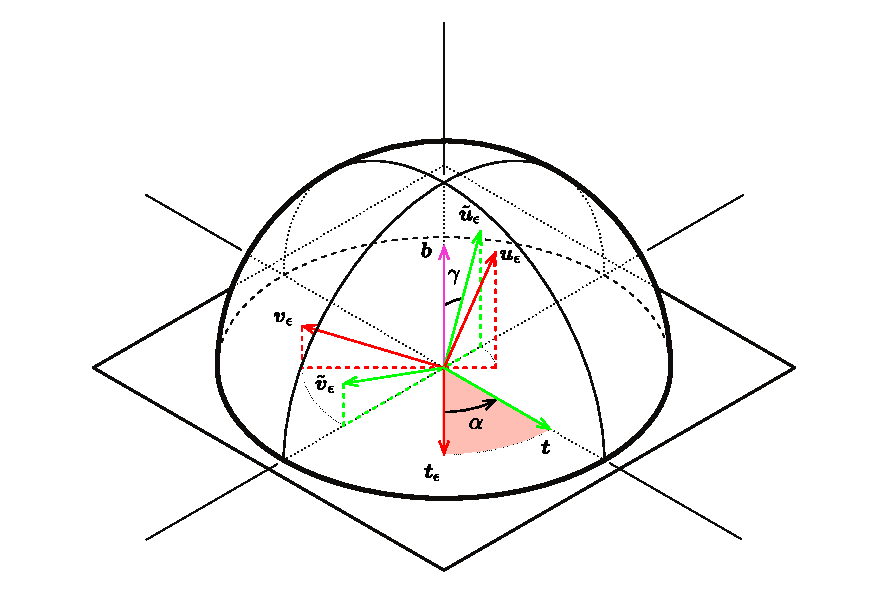
\includegraphics[width=\textwidth]{rotation_B.pdf}
	\captionof{figure}[Measuring the variation of parallel transport : rotation of angle $\alpha_\epsilon$.]{Measuring the variation of parallel transport ($\alpha_\epsilon$). $\tilde{F}_\epsilon$ is obtained by parallel tranpsporting $F_\epsilon$ from $\vect{t}_\epsilon$ to $\vect{t}$. This operation could be seen as a rotation around the axis $\vect{b} = \vect{t}_\epsilon \times \vect{t}$ by an angle $\alpha_\epsilon$.}
	\label{fig:rot_a}
%
	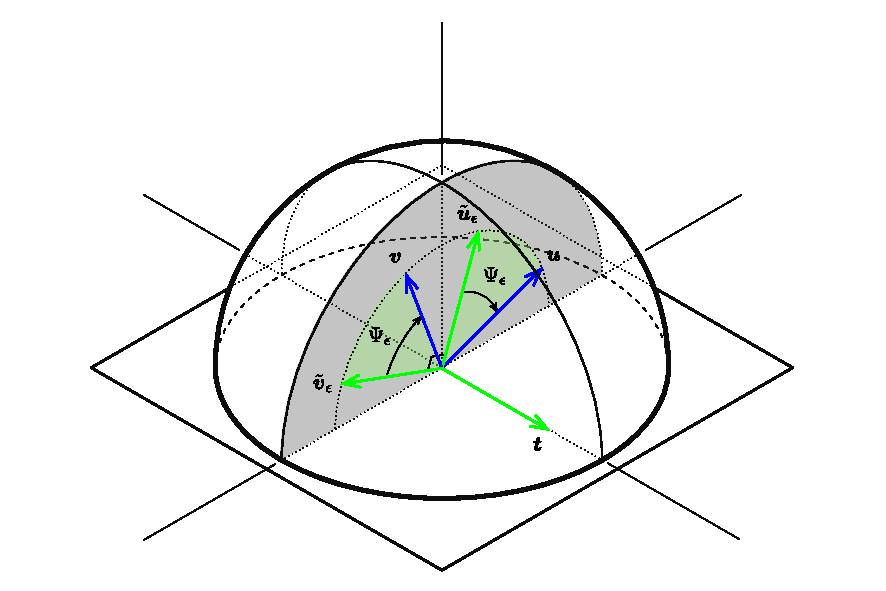
\includegraphics[width=\textwidth]{rotation_A.pdf}
	\captionof{figure}[Measuring the variation of parallel transport : rotation of angle $\Psi_\epsilon$.]{Measuring the variation of parallel transport ($\Psi_\epsilon$). $F$ is obtained by rotating $\tilde{F}_\epsilon$ around $\vect{t}$ by an angle $\Psi_\epsilon$.}
	\label{fig:rot_b}
\end{figure}

This variation is closely related to the writhe of closed curves. As explained by \citef{Fuller1978} when parallel transporting an adapted frame around a closed curve it might not realigned with itself after one complete loop. This \textquote{lack of alignement} is directly measured by the change of writhe which can be computed with Fuller's Formula~\cite{Fuller1978}.

Note that the derivative of $\theta$ with respect to $\vect{x}$ can be evaluated by the change of writhe in the curve as suggested in~\cite{deVries2005}. This approach is completly equivalent.

One can also see this lack of alignement in terms of rotation. Parallel transport being a propagation of frame from $s = 0$, the cumulated rotation of the Bishop frame from the deformed configuration around the initial configuration at arc length $s$ is the cumulated angle of rotation of $\vect{u}[\vect{x} + \lambda\vect{h}_x]$ around $\vect{d}_3[\vect{x}]$. Recalling that the rotation rate of $\vect{u}[\vect{x} + \lambda\vect{h}_x]$ is $\vect{\kappa b}[\vect{x} + \lambda\vect{h}_x]$ by definition of zero-twisting frame, one can write~:
\begin{equation}
	\Psi_\epsilon[\vect{x}](s) =
	-\int_0^s \vect{\kappa b}[\vect{x} + \lambda\vect{h}_x] \cdot \vect{d}_3[\vect{x}] \,dt
\end{equation}
The calculation of $\vect{\kappa b}[\vect{x} + \lambda\vect{h}_x]$ is straight forward from the definition of the curvature binormal (see \cref{eq:kb2})~:
\begin{equation}
	\begin{aligned}
	\vect{\kappa b}[\vect{x} + \lambda\vect{h}_x]
	&= (\vect{x} + \lambda\vect{h}_x)' \times (\vect{x} + \lambda\vect{h}_x)'' \\
	&= \vect{\kappa b}[\vect{x}] + \lambda(\vect{x}'\times\vect{h}''_x + \vect{h}'_x\times\vect{x}'') + \lambda^2(\vect{h}'_x \times \vect{h}''_x) \\
	&= \vect{\kappa b}[\vect{x}] + \lambda(\vect{x}'\times\vect{h}''_x + \vect{h}'_x\times\vect{x}'') + o(\lambda)
	\end{aligned}
\end{equation}
Thus, reminding that $\vect{d}_3[\vect{x}] = \vect{x}'$ and $\vect{\kappa b}[\vect{x}]\cdot\vect{d}_3[\vect{x}] = 0$, and using the invariance of circular product by cyclic permutation, one can express~:
\begin{equation}
	\begin{aligned}
		\Psi_\epsilon[\vect{x}](s)
		&= -\int_0^s \vect{\kappa b}[\vect{x} + \lambda\vect{h}_x] \cdot \vect{d}_3[\vect{x}] \,dt\\
		&= - \lambda \int_0^s (\vect{x}'\times\vect{h}''_x + \vect{h}'_x\times\vect{x}'') \cdot \vect{x}' \,dt + o(\lambda)\\
		&= - \lambda \int_0^s \vect{\kappa b}[\vect{x}]\cdot\vect{h}'_x \,dt + o(\lambda)\\
	\end{aligned}
\end{equation}
By integration by parts and dropping the implicit reference to $\vect{x}$ in the notation, $\Psi_\epsilon(s)$ can be rewritten as~:
\begin{equation}
	\begin{aligned}
		\Psi_\epsilon(s)
		&= - \lambda \int_0^s \vect{\kappa b}\cdot\vect{h}'_x \,dt + o(\lambda)\\
		&=  - \lambda \left(\big[\vect{\kappa b} \cdot  \vect{h}_x \big]_0^s - \int_0^s \vect{\kappa b}' \cdot  \vect{h}_x \,dt\right) + o(\lambda)\\
		&= - \lambda \left(\int_0^s \left(\left(\delta_s-\delta_0\right)\vect{\kappa b} - \vect{\kappa b}'\right)\cdot  \vect{h}_x \,dt\right) + o(\lambda)\\
		&= - \lambda \left(\int_0^L \left(\left(\delta_s-\delta_0\right)\vect{\kappa b} - (1-H_s)\vect{\kappa b}'\right)\cdot  \vect{h}_x \,dt\right) + o(\lambda)
	\end{aligned}
\label{eq:psi}
\end{equation}
where $\delta_s$ and $H_s$ are the Dirac function and the Heaviside step function centered at $s$~:
\begin{subequations}
	\begin{alignat}{1}
		H_s &: t \mapsto \left\{\begin{array}{c}0  , \quad t<s \\1  , \quad t\geqslant s \end{array}\right.
		\\[1em]
		\delta_s &: t \mapsto \delta(t-s)
	\end{alignat}
\end{subequations}
Note that, as expected, $\Psi_\epsilon(s)$ is in first order of $\lambda$ and thus gets negligible when $\lambda$ tends to zero, that is to say when the perturbation of $\vect{x}$ is infinitesimal~:
\begin{equation}
	\lim_{\lambda \to 0} \Psi_\epsilon(s) = 0
	\label{eq:lim_psi}
\end{equation}



\subsubsection{Calculation of $\alpha_\epsilon$}

Recall that $\tilde{F}_\epsilon$ is obtained by parallel tranpsporting $F_\epsilon$ from $\vect{t}_\epsilon$ to $\vect{t}$.
$\tilde{F}_\epsilon$ results from the rotation of $F_\epsilon$ around $\vect{b} = \vect{t}_\epsilon \times \vect{t}$ by an angle $\alpha_\epsilon$.

Recall from \cref{eq:axialstrain} that because the rod is supposed to be inextensible, $\vect{t}_\epsilon$ stays collinear to $\vect{t}$, at first order in $\lambda$, for an infinitesimal perturbation of the centerline~:
\begin{equation}
		\|\vect{t}\| = \|\vect{t}_\epsilon\| = 1
		\Rightarrow  (\vect{x}+\vect{\epsilon})' \cdot (\vect{x}+\vect{\epsilon})' = 1
		\Leftrightarrow  \vect{x}'\cdot\vect{\epsilon}' = - \tfrac{\lambda^2}{2}\|\vect{h}_x'\|^2
\end{equation}
Which yields~:
\begin{equation}
		\cos \alpha_\epsilon = \vect{t} \cdot \vect{t}_\epsilon = \vect{x}' \cdot (\vect{x}+\vect{\epsilon})'
		= 1 + \vect{x}' \cdot \vect{\epsilon}'
		= 1 - \tfrac{\lambda^2}{2}\|\vect{h}_x'\|^2
\end{equation}
Remark that the second order of the developpement is also accessible and can lead to the computation of the hessian of the system, which might be useful for improving the convergence of the minimization algorithm~:
\begin{subequations}
	\begin{alignat}{2}
		&\cos \alpha_\epsilon = 1 - \tfrac{\lambda^2}{2}\|\vect{h}_x'\|^2
		\\
		&\sin \alpha_\epsilon = \sqrt{1-\cos^2 \alpha_\epsilon} = \lambda\|\vect{h}_x'\| + o(\lambda^2)
		\\
		&\sin^2 {\alpha_\epsilon}{/2} = \tfrac{\lambda^2}{4}\|\vect{h}_x'\|^2
	\end{alignat}
\end{subequations}
Finally, it's possible to conclude that $\alpha_\epsilon(s)$ is in first order of $\lambda$ and thus gets negligible when $\lambda$ tends to zero~:
\begin{equation}
	\lim_{\lambda \to 0} \alpha_\epsilon(s) = 0
	\label{eq:lim_alpha}
\end{equation}

%\begin{figure}[t]
%\centering
%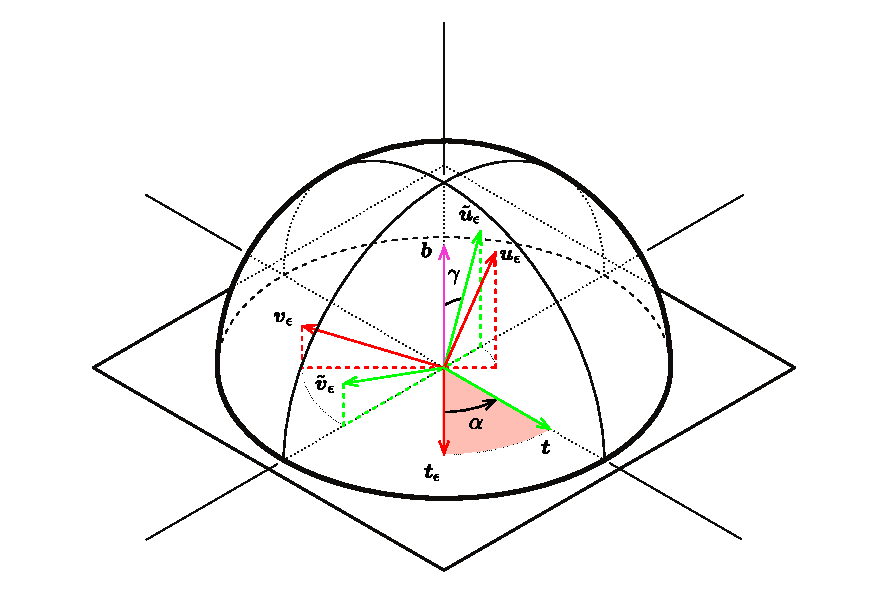
\includegraphics[width=\linewidth]{rotation_B.pdf}
%\captionof{figure}[]{$\tilde{F}_\epsilon$ is obtained by parallel tranpsporting $F_\epsilon$ from $\vect{t}_\epsilon$ to $\vect{t}$. This operation could be seen as a rotation around $\vect{t}_\epsilon \times \vect{t}$ of an angle $\alpha$.}
%\label{fig:varbishop}
%\end{figure}

\subsubsection{Aligning $\tilde{F}_\epsilon$ towards $F_\epsilon$}
Recall that aligning $\tilde{F}_\epsilon$ over $F$ is nothing but a rotation around $\vect{t}$ by an angle $\Psi_\epsilon$. This leads to~:
\begin{subequations}
%	\left\{
	\begin{alignat}{5}
		&\vect{\tilde{u}}_\epsilon &&=& \cos{\Psi_\epsilon}\;\vect{u} &+ \sin{\Psi_\epsilon}\;\vect{v}\\
		&\vect{\tilde{v}}_\epsilon &&=& -\sin{\Psi_\epsilon}\;\vect{u} &+ \cos{\Psi_\epsilon}\;\vect{v}
	\end{alignat}
%	\right.
\end{subequations}

\subsubsection{Aligning $F_\epsilon$ towards $\vect{t}$}

Recall that $\tilde{F}_\epsilon$ is obtained by parallel tranpsporting $F_\epsilon$ from $\vect{t}_\epsilon$ to $\vect{t}$. This operation could be seen as a rotation around $\vect{t}_\epsilon \times \vect{t}$ of an angle $\alpha_\epsilon$. Where~:
\begin{equation}
	\vect{b} = \vect{t}_\epsilon \times \vect{t}
	 = \cos{\gamma}\;\vect{\tilde{u}}_\epsilon + \sin{\gamma}\;\vect{\tilde{v}}_\epsilon
	 = \cos{\gamma}\;\vect{u}_\epsilon + \sin{\gamma}\;\vect{v}_\epsilon
\end{equation}
Expressing $F_\epsilon$ on the basis $\tilde{F}_\epsilon$ gives for $\vect{u}_\epsilon$ and $\vect{v}_\epsilon$~:
\begin{subequations}
\begin{alignat}{3}
		&\vect{u}_\epsilon &&= \sin{\gamma}\;\vect{b} + \cos{\gamma}\;\big(\sin{\alpha_\epsilon}\;\vect{\tilde{t}}
	+ \cos{\alpha_\epsilon}\;(\cos{\gamma}\;\vect{\tilde{u}_\epsilon}
	- \sin{\gamma}\;\vect{\tilde{v}_\epsilon})\big)
		\\
		&\vect{v}_\epsilon &&= \cos{\gamma}\;\vect{b} + \sin{\gamma}\;\big(-\sin{\alpha_\epsilon}\;\vect{\tilde{t}}
	+ \cos{\alpha_\epsilon}\;(\sin{\gamma}\;\vect{\tilde{u}_\epsilon}
	- \cos{\gamma}\;\vect{\tilde{v}_\epsilon})\big)
\end{alignat}
\end{subequations}
Which can be rearranged in~:
\begin{subequations}
\begin{alignat}{1}
	&\vect{u}_\epsilon = \phantom{-}\cos{\gamma}\sin{\alpha_\epsilon}\;\vect{t} 
	+ (\cos{\alpha_\epsilon}\cos^2{\gamma} + \cos^2{\gamma})\vect{\tilde{u}_\epsilon} 
	+ \phantom{(}\sin{\gamma}\cos{\gamma}\;(1-\cos{\alpha_\epsilon})\vect{\tilde{v}_\epsilon}
		\\
	&\vect{v}_\epsilon = -\sin{\gamma}\sin{\alpha_\epsilon}\;\vect{t} 
	+ \phantom{.}\cos{\gamma}\sin{\gamma}\;(1-\cos{\alpha_\epsilon})\vect{\tilde{u}_\epsilon} 
	+ (\cos^2{\gamma} + \cos{\alpha_\epsilon}\sin^2{\gamma})\vect{\tilde{v}_\epsilon}
\end{alignat}
\end{subequations}

\subsubsection{Variation of the Bishop frame with respect to $x$}
Finally, one can express $F_\epsilon$ on the basis $F$ as the composition of two rotations~:
\begin{subequations}
	\begin{gather}
	\vect{u}_\epsilon =
	\begin{bmatrix}
		1 & 0 & 0 \\
		0 & \cos{\Psi_\epsilon} & -\sin{\Psi_\epsilon} \\
		0 & \sin{\Psi_\epsilon} & \cos{\Psi_\epsilon}
	\end{bmatrix}
	\begin{bmatrix}
		\cos{\gamma}\sin{\alpha_\epsilon} \\
		1-2\cos^2{\gamma}\sin^2{\alpha_\epsilon/2} \\
		2\sin{\gamma}\cos{\gamma}\sin^2{\alpha_\epsilon/2}
	\end{bmatrix}
	=
	\begin{bmatrix}
		\alpha_\epsilon\cos{\gamma}\\
		1 \\
		\Psi_\epsilon
	\end{bmatrix}
	+ o(\lambda)
	\\
	\vect{v}_\epsilon =
	\begin{bmatrix}
		1 & 0 & 0 \\
		0 & \cos{\Psi_\epsilon} & -\sin{\Psi_\epsilon} \\
		0 & \sin{\Psi_\epsilon} & \cos{\Psi_\epsilon}
	\end{bmatrix}
	\begin{bmatrix}
		-\sin{\gamma}\sin{\alpha_\epsilon} \\
		2\sin{\gamma}\cos{\gamma}\sin^2{\alpha_\epsilon/2} \\
		1-2\sin{\gamma}^2\sin^2{\alpha_\epsilon/2}
	\end{bmatrix}
	=
	\begin{bmatrix}
		-\alpha_\epsilon\sin{\gamma}\\
		-\Psi_\epsilon \\
		1
	\end{bmatrix}
	+ o(\lambda)
	\end{gather}
\end{subequations}

%\begin{equation}
%
%\end{equation}
Here, the expressions have been developed in first order of $\lambda$. It has been prooved in \cref{eq:lim_alpha,eq:lim_psi} that $\alpha_\epsilon$ and $\Psi_\epsilon$ tend toward zero when the perturbation of the centerline is infinitesimal.

Finally, one can express the variation of the material directors with respect to an infinitesimal variation of rod's centerline by~:
\begin{subequations}
\begin{alignat}{7}
		&\vect{u}_\epsilon &&=& \alpha_\epsilon\cos{\gamma}\;\vect{t} + \vect{u} + \Psi_\epsilon\vect{v} &+ o(\lambda)
		\\
		&\vect{v}_\epsilon &&=& -\alpha_\epsilon\sin{\gamma}\;\vect{t} + \vect{v} - \Psi_\epsilon\vect{u} &+ o(\lambda)
\end{alignat}
\end{subequations}

\subsubsection{Variation of the material frame with respect to $\vect{x}$}
Recalling the expression of the material frame expressed in the reference Bishop frame, it's now easy to deduce the variation of material frame with respect to a variation of the rod's centerline~:
\begin{subequations}
		\begin{alignat}{7}
			&\vect{d}_1[\vect{x}+\lambda \vect{h}_x] &&=&
			\cos{\theta} \; \vect{u}_\epsilon &+ \sin{\theta} \; \vect{v}_\epsilon\\
			&\vect{d}_2[\vect{x}+\lambda \vect{h}_x] &&=&
			-\sin{\theta} \; \vect{u}_\epsilon &+ \cos{\theta} \; \vect{v}_\epsilon
		\end{alignat}
\end{subequations}
Which leads according to the previous equation to~:
\begin{subequations}
	\begin{alignat}{7}
		&\vect{d}_1[\vect{x}+\lambda \vect{h}_x] &&=& \vect{d}_1[\vect{x}] + \Psi_\epsilon\vect{d}_2[\vect{x}] + \alpha_\epsilon\cos{(\theta-\gamma)}\;\vect{t}[\vect{x}] 
		&+ o(\lambda) \\
		&\vect{d}_2[\vect{x}+\lambda \vect{h}_x] &&=& \vect{d}_2[\vect{x}] - \Psi_\epsilon\vect{d}_1[\vect{x}] - \alpha_\epsilon\sin{(\theta+\gamma)}\;\vect{t}[\vect{x}] 
		&+ o(\lambda)
		\end{alignat}
\end{subequations}

\subsection{Derivative of the vector of material curvatures with respect to $x$}

It is now straightforward from the previous section to express the variation of the material curvatures with respect to a variation $\vect{\epsilon} =\lambda \vect{h}_x$ of $\vect{x}$ while $\theta$ remains unchanged~:
\begin{subequations}
	\begin{alignat}{7}
		&(\vect{x}+\lambda \vect{h}_x)'' \cdot \vect{d}_1[\vect{x}+\lambda \vect{h}_x] && = 
			(\vect{x}''+\lambda \vect{h}_x'')
			\\ &&&\phantom{=}\cdot\big(\vect{d}_1 + \Psi_\epsilon\vect{d}_2
			+ \alpha_\epsilon\cos{(\theta-\gamma)}\;\vect{t} + o(\lambda)\big)  \nonumber
		\\[1em]
		&(\vect{x}+\lambda \vect{h}_x)'' \cdot \vect{d}_2[\vect{x}+\lambda \vect{h}_x] && = 
			(\vect{x}''+\lambda \vect{h}_x'')
			\\ &&&\phantom{=}\cdot\big(\vect{d}_2 - \Psi_\epsilon\vect{d}_1
			- \alpha_\epsilon\sin{(\theta+\gamma)}\;\vect{t} + o(\lambda)\big) \nonumber
	\end{alignat}
\end{subequations}
Thus, recalling that $\vect{x}''\cdot\vect{d}_3 = 0$ and that $\alpha_\epsilon$ and $\Psi_\epsilon$ are first order quantities in $\lambda$~:
\begin{subequations}
	\begin{gather}
		(\vect{x}+\lambda \vect{h}_x)'' \cdot \vect{d}_1[\vect{x}+\lambda \vect{h}_x] = 					\vect{x}''\cdot\vect{d}_1 + \Psi_\epsilon\vect{x}''\cdot\vect{d}_2 + \lambda \vect{h}_x''\cdot\vect{d}_1 + o(\lambda)\\
		(\vect{x}+\lambda \vect{h}_x)'' \cdot \vect{d}_2[\vect{x}+\lambda \vect{h}_x] =
				\vect{x}''\cdot\vect{d}_2 - \Psi_\epsilon\vect{x}''\cdot\vect{d}_1 +  \lambda \vect{h}_x''\cdot\vect{d}_2 + o(\lambda)
	\end{gather}
\end{subequations}
Which finally leads to~:
\begin{equation}
		\vect{\omega}[\vect{x}+\lambda \vect{h}_x]  =
		\vect{\omega}[\vect{x}] - \Psi_\epsilon\mat{J}\vect{\omega}[\vect{x}]+\lambda
		\begin{bmatrix*}[r]
			-\vect{h}_x''\cdot\vect{d}_2\\
			\vect{h}_x''\cdot\vect{d}_1\\
		\end{bmatrix*} + o(\lambda)
\end{equation}
Reminding the expression of $\Psi_\epsilon$ computed in \cref{eq:psi}, one can express the derivative of the vector of material curvatures with respect to $\vect{x}$ as~:
\begin{equation}
			\pdiffof{x}{\vect{\omega}}{s}{\vect{h}_x}
	= 	\left(\int_0^L \left(\left(\delta_s-\delta_0\right)\vect{\kappa b} - (1-H_s)\vect{\kappa b}'\right)\cdot  \vect{h}_x \,dt\right)\mat{J}\vect{\omega}+
		\begin{bmatrix*}[r]
			-{\vect{d}_2}^T\\
			{\vect{d}_1}^T\\
		\end{bmatrix*}\cdot \vect{h}_x''
\label{eq:dwdx}
\end{equation}
Here, we have introduce a condensed matrix notation to write $\begin{bmatrix*}[r] -{\vect{d}_2}^T\\ {\vect{d}_1}^T\\ \end{bmatrix*}$ as a 2x3 matrix. The entries of the first line are $-{\vect{d}_2}^T = \begin{bmatrix} 0,\;0,\;-1 \end{bmatrix}$ while the entries of the second line are ${\vect{d}_1}^T = \begin{bmatrix} 0,\;1,\;0 \end{bmatrix}$. Thus, the matrix entries in the material frame coordinate system are given by~:
\begin{equation}
	\begin{bmatrix*}[r] -{\vect{d}_2}^T\\ {\vect{d}_1}^T \end{bmatrix*}
	= 
	\begin{bmatrix} 0 & 0 & -1 \\ 0 & 1 & 0 \end{bmatrix}
\end{equation}
Remark also how the scalar product $\vect{h}_x''\cdot\vect{d}_2$ in vector notation is treated as a product in matrix notation~: ${\vect{d}_2}^T \cdot \vect{h}_x'' =  {(\vect{h}_x'')}^T \cdot {\vect{d}_2}$.

\subsection{Computation of the forces acting on the centerline}
The distributed internal forces acting on the centerline are given by the functional derivative of the elastic energy with respect to $\vect{x}$, which can be decomposed into~:
\begin{equation}
	\begin{aligned}
	\scalar{-\vect{f}(s)}{\vect{h}_x} 
	&= \pdiffof{x}{\mathcal{E}}{s}{\vect{h}_x} \\
	&= \pdiffof{x}{\mathcal{E}_b}{s}{\vect{h}_x} + \pdiffof{x}{\mathcal{E}_t}{s}{\vect{h}_x} \\
%	&= \pdiffof{x}{\mathcal{E}_b[\vect{\omega}[\vect{x}]]}{s}{\vect{h}_x} + \pdiffof{x}{\mathcal{E}_t[\vect{x}]}{s}{\vect{h}_x} \\
	\end{aligned}
\label{eq:dEdx_def}
\end{equation}

\subsubsection{Derivative of the torsion energy with respect to $x$}

Recall that the torsion energy only depends on $\theta$ which is independent of $x$. Thus $\mathcal{E}_t$ is independent of $x$ and~:
\begin{equation}
	\pdiffof{x}{\mathcal{E}_t[\vect{x}]}{s}{\vect{h}_x}
		= \frac{d}{d\lambda} \mathcal{E}_t[\vect{x} + \lambda \vect{h}_x]\Bigr|_{\lambda = 0} = 0
\label{eq:dEtdx}
\end{equation}

\subsubsection{Derivative of the bending energy with respect to $x$}
To compute the partial derivative of $\mathcal{E}_b$ with respect to $\vect{x}$ we first calculate the derivative of $\mathcal{E}_b$ with respect to $\vect{\omega}$~:
\begin{equation}
	\pdiffof{\omega}{\mathcal{E}_b[\vect{\omega}]}{s}{\vect{h}_\omega}
		= \frac{d}{d\lambda} \mathcal{E}_b[\vect{\omega} + \lambda \vect{h}_\omega]\Bigr|_{\lambda = 0}
		= \int_{0}^{L} (\vect{\omega} - \rconf{\vect{\omega}})^T \mat{B} \cdot \vect{h}_\omega \;dt
\label{eq:dEbdw}
\end{equation}
Then, we calculate the partial derivative of $\mathcal{E}_b$ with respect to $\vect{x}$ from the chain rule and with \cref{eq:dwdx,eq:dEbdw}~:
\begin{equation}
	\pdiffof{x}{\mathcal{E}_b[\vect{\omega}[\vect{x}]]}{s}{\vect{h}_x}
	= \pdiffof{\omega}{\mathcal{E}_b[\vect{\omega}]}{s}{(\pdiffof{x}{\vect{\omega}[\vect{x}]}{s}{\vect{h}_x})}
	= \mathcal{A} +\mathcal{B}+\mathcal{C}
\label{eq:dEdx}
\end{equation}
where $\mathcal{A} $, $\mathcal{B}$ and $\mathcal{C}$ are given by~:
\begin{subequations}
	\begin{gather}
	\mathcal{A} = \int_{0}^{L} (\vect{\omega} - \rconf{\vect{\omega}})^T \mat{B}
	\begin{bmatrix*}[r]
		-{\vect{d}_2}^T\\
		{\vect{d}_1}^T\\
	\end{bmatrix*}\cdot \vect{h}_x'' \;dt \\
	\mathcal{B} =
	\int_{t=0}^{L} (\vect{\omega} - \rconf{\vect{\omega}})^T \mat{B}\mat{J}\vect{\omega}
	\left(\int_{u=0}^L \left(\delta_t-\delta_0\right)\vect{\kappa b}\cdot  \vect{h}_x \;du\right)
	\;dt\\
	\mathcal{C} =
	\int_{t=0}^{L} -(\vect{\omega} - \rconf{\vect{\omega}})^T \mat{B}\mat{J}\vect{\omega}
	\left(\int_{u=0}^L \left(1-H_t\right)\vect{\kappa b}'\cdot  \vect{h}_x \;du\right)
	\;dt
	\end{gather}
\end{subequations}

Calculus of $\mathcal{A}$~:
\begin{equation}
	\mathcal{A}
	= \int_{0}^{L} (\vect{\omega} - \rconf{\vect{\omega}})^T \mat{B}
		\begin{bmatrix*}[r]
			-{\vect{d}_2}^T\\
			{\vect{d}_1}^T\\
		\end{bmatrix*}\cdot \vect{h}_x'' \;dt \\
\label{eq:calcA}
\end{equation}
One can remark that the (row) vector found in \cref{eq:calcA} can be rewritten as~: \footnote{Here, we mix up vector and matrix notations. The matrix form of a vector is given by the components of the vector in the material frame coordinate system. For instance, $({\vect{d}_3} \times \vect{M}^{\perp})^T$ is a row vector that writes in its matrix form~: $\begin{bmatrix} 0,\;-M2,\;M1 \end{bmatrix}$.}
\begin{equation}
	\left(\vect{\omega} - \rconf{\vect{\omega}}\right)^T \mat{B}
		\begin{bmatrix*}[r]
			-{\vect{d}_2}^T\\
			{\vect{d}_1}^T\\
		\end{bmatrix*}
	=  M_2{\vect{d}_1}^T - M_1{\vect{d}_2}^T
	= - ({\vect{d}_3} \times \vect{M}^{\perp})^T
\end{equation}
Thus,  $\mathcal{A}$ could be rewritten in it's vectoriel form~:
\begin{equation}
	\begin{aligned}
	\mathcal{A}
	& = -\int_{0}^{L} ({\vect{d}_3} \times \vect{M}^{\perp}) \cdot \vect{h}_x'' \;dt \\
	& = -\left[\left({\vect{d}_3} \times \vect{M}^{\perp}\right) \cdot \vect{h}_x'\right]_0^L
		+ \int_{0}^{L} \left({\vect{d}_3} \times \vect{M}^{\perp}\right)'\cdot \vect{h}_x' \;dt \\
	& = -\left[\left({\vect{d}_3} \times \vect{M}^{\perp}\right) \cdot \vect{h}_x'\right]_0^L
		+ \int_{0}^{L} \left(
			\left({\vect{d}_3} \times {\vect{M}^{\perp}}'\right) \cdot \vect{h}_x'
			+ \left({\vect{h}'_x} \times \vect{d}_3'\right) \cdot \vect{M}^{\perp}
			 \right)\;dt \\
	\end{aligned}
\end{equation}
Recall that from \cref{eq:axialstrain} that $\vect{h}'_x \cdot \vect{d}_3 = 0$  and from \cref{eq:mf_motion} that $\vect{d}'_3 \cdot \vect{d}_3 = 0$. Hence, $\vect{h}'_x \times \vect{d}_3'$ is colinear to $\vect{d}_3$. Or by definition $\vect{M}^{\perp}$ is orthogonal to $\vect{d}_3$. Thus, $\left({\vect{h}'_x} \times \vect{d}_3'\right) \cdot \vect{M}^{\perp} = 0$.
Finally, after a second integration by parts~:
\begin{equation}
	\begin{aligned}
	\mathcal{A}
	& = -\left[\left({\vect{d}_3} \times \vect{M}^{\perp}\right) \cdot \vect{h}_x'\right]_0^L
		+ \int_{0}^{L} \left(
			{\vect{d}_3} \times {\vect{M}^{\perp}}'\right) \cdot \vect{h}_x'
			 \;dt \\
	& = 	\phantom{-}\left[
			({\vect{d}_3} \times {\vect{M}^{\perp}}') \cdot \vect{h}''_x\
			- ({\vect{d}_3} \times \vect{M}^{\perp}) \cdot \vect{h}_x'
		\right]_0^L
		- \int_{0}^{L} \left({\vect{d}_3} \times {\vect{M}^{\perp}}'\right)' \cdot \vect{h}_x \;dt \\
	\end{aligned}
\label{eq:A}
\end{equation}
Calculus of $\mathcal{B}$~:
\begin{equation}
	\begin{aligned}
	\mathcal{B} &=
	\int_{t=0}^{L} (\vect{\omega} - \rconf{\vect{\omega}})^T \mat{B}\mat{J}\vect{\omega}
	\left(\int_{u=0}^L \left(\delta_t-\delta_0\right)\vect{\kappa b}\cdot  \vect{h}_x \,du\right)
	\;dt
	\\
	&=
	-\left(\vect{\kappa b}\cdot\vect{h}_x\right)(0) \int_{t=0}^{L} (\vect{\omega} - \rconf{\vect{\omega}})^T \mat{B}\mat{J}\vect{\omega}\;dt
	+
	\int_{t=0}^{L} (\vect{\omega} - \rconf{\vect{\omega}})^T \mat{B}\mat{J}\vect{\omega}
	\vect{\kappa b}\cdot\vect{h}_x
	\;dt
	\end{aligned}
\label{eq:B}
\end{equation}
Calculus of $\mathcal{C}$~:
\begin{equation}
	\begin{aligned}
	\mathcal{C} &=
	\int_{t=0}^{L} -(\vect{\omega} - \rconf{\vect{\omega}})^T \mat{B}\mat{J}\vect{\omega}
	\left(\int_{u=0}^L \left(1-H_t\right)\vect{\kappa b}'\cdot  \vect{h}_x \;du\right)
	\;dt
	\\
	&=
	\int_{u=0}^{L}\int_{t=u}^{L}-\left((\vect{\omega} - \rconf{\vect{\omega}})^T \mat{B}\mat{J}\vect{\omega}\right)(t)
	\left(\vect{\kappa b}'\cdot \vect{h}_x\right)(u) \;dt\;du
	\\
	&=
	\int_{u=0}^{L}-\left(\int_{t=u}^{L}(\vect{\omega} - \rconf{\vect{\omega}})^T \mat{B}\mat{J}\vect{\omega}\;dt\right)
	\left(\vect{\kappa b}'\cdot \vect{h}_x\right)\;du
	\\
	\end{aligned}
\label{eq:C}
\end{equation}
By several integration by parts, using Fubini's theorem once and supposing that the terms vanishes at $s=0$ and $s=L$~:
\begin{equation}
	\begin{aligned}
	\mathcal{B}+\mathcal{C} &=
	\int_{t=0}^{L} \left(
	(\vect{\omega} - \rconf{\vect{\omega}})^T \mat{B}\mat{J}\vect{\omega}
	\vect{\kappa b}
	-
	\left(\int_{u=t}^{L}(\vect{\omega} - \rconf{\vect{\omega}})^T \mat{B}\mat{J}\vect{\omega}\;du\right)
	\vect{\kappa b}'
	\right)\cdot \vect{h}_x \;dt\\
	&=
	\int_{t=0}^{L} \left(
	-\left(\int_{u=t}^{L}(\vect{\omega} - \rconf{\vect{\omega}})^T \mat{B}\mat{J}\vect{\omega}\;du\right)'
	\vect{\kappa b}
	-
	\left(\int_{u=t}^{L}(\vect{\omega} - \rconf{\vect{\omega}})^T \mat{B}\mat{J}\vect{\omega}\;du\right)
	\vect{\kappa b}'
	\right)\cdot \vect{h}_x \;dt\\
	&=
	\int_{t=0}^{L} \left(
	-\left(\int_{u=t}^{L}(\vect{\omega} - \rconf{\vect{\omega}})^T \mat{B}\mat{J}\vect{\omega}\;du\right)
	\vect{\kappa b}
	\right)'\cdot \vect{h}_x \;dt\\
	\end{aligned}
\end{equation}
Which can be rewritted using the quasi-static hypothesis \cref{eq:quasistat}~:
\begin{equation}
	\begin{aligned}
	\mathcal{B}+\mathcal{C}
	&=
	\int_{t=0}^{L} \left(
	-\left(\int_{u=t}^{L}(\vect{\omega} - \rconf{\vect{\omega}})^T \mat{B}\mat{J}\vect{\omega}\;du\right)
	\vect{\kappa b}
	\right)'\cdot \vect{h}_x \;dt\\
	&=
	\int_{t=0}^{L} \left(
	-\left(
	\int_{u=t}^{L}\beta(\theta' -{\rconf{\theta}'})(\delta_L-\delta_0) - \left(\beta(\theta' -{\rconf{\theta}'})\right)'\;du
	\right)
	\vect{\kappa b}
	\right)'\cdot \vect{h}_x \;dt\\
	&=
	\int_{t=0}^{L} \left(
	-\left(
	\beta(\theta' -{\rconf{\theta}'})(L) - \left[\beta(\theta' -{\rconf{\theta}'})\right]_t^L
	\right)
	\vect{\kappa b}
	\right)'\cdot \vect{h}_x \;dt\\
		&=
	\int_{t=0}^{L} -\left(
	\beta(\theta' -{\rconf{\theta}'})
	\vect{\kappa b}
	\right)'\cdot \vect{h}_x \;dt\\
	\end{aligned}
\label{eq:BC}
\end{equation}
Finally, combining \cref{eq:A,eq:BC} into \cref{eq:dEdx} yields~:
\begin{equation}
		\pdiffof{x}{\mathcal{E}_b[\vect{\omega}[\vect{x}]]}{s}{\vect{h}_x}
		=
		\int_{0}^{L} \left(
		- \left({\vect{d}_3} \times {\vect{M}^{\perp}}'\right)'
		- \left(\beta(\theta' -{\rconf{\theta}'}) \vect{\kappa b}\right)'
		\right)\cdot \vect{h}_x \;dt\\
\label{eq:dEbdx}
\end{equation}

\subsubsection{Internal forces}
The gradient of the elastic energy with respect to $\vect{x}$ is obtained from \cref{eq:dEdx_def} with \cref{eq:dEtdx,eq:dEbdx}~:
\begin{equation}
	\begin{aligned}
	\scalar{-\vect{f}(s)}{\vect{h}_x} &= \pdiffof{x}{\mathcal{E}}{s}{\vect{h}_x}
		=
		- \int_{0}^{L} \left(
		\left({\vect{d}_3} \times {\vect{M}^{\perp}}'\right)'
		+ \left(\beta(\theta' -{\rconf{\theta}'}) \vect{\kappa b}\right)'
		\right)\cdot \vect{h}_x \;dt\\
	\end{aligned}
\end{equation}
Finally, we can conclude on the expression of the distributed internal forces acting on the centermine~:
\begin{equation}
	\vect{f}(s) = \left({\vect{d}_3} \times {\vect{M}^{\perp}}'(s) + \beta\left(\theta' -{\rconf{\theta}'}\right) \vect{\kappa b}\right)'(s)
\end{equation}
Remark that this expression can be rewritten thanks to \cref{eq:Q2} as~:
\begin{equation}
	\vect{f}(s) = \left({\vect{d}_3} \times {\vect{M}^{\perp}}' + Q \vect{\kappa b}\right)'(s)
\label{eq:fint}
\end{equation}

\section{Shear force acting on the rod}\label{sec:fmint}
From \cref{eq:fint,eq:mint} we deduce the internal shear force and distributed twisting moment acting on the rod~:
\begin{subequations}
	\begin{alignat}{2}
	\vect{F} &=  {\vect{d}_3} \times \vect{M}' \label{eq:Fshear}\\
	m &= Q' +  \kappa_1\;M_2 - \kappa_2\; M_1
	\end{alignat}
\end{subequations}
Remark that we fall back on the static member of the dynamical equations of rods in Kirchhoff's theory (see \cref{eq:motion}). Hence, we have proved the equivalence between the present approach (based on the calculus of variations and the formulation of an elastic energy) and a more direct approach from the well-established Kirchhoff equations.\footnote{It is easy from \cref{eq:Fshear} to retrieve \cref{eq:motion_4,eq:motion_5} considering that~: 
\begin{equation*}
	\begin{aligned}
	{\vect{d}_3} \times \vect{M}'
	&= \vect{d}_3 \times ({\vect{M}^{\perp}}' + (Q\;\vect{d}_3)') \\
	&= \vect{d}_3 \times ({\vect{M}^{\perp}}' + Q\;\vect{d}'_3) \\
	&=  \vect{d}_3 \times ({\vect{M}^{\perp}}' + Q\;(\tau \vect{d}_3 + \vect{\kappa b}) \times \vect{d}_3) \\
	&= \vect{d}_3 \times {\vect{M}^{\perp}}' +  Q\;\vect{\kappa b}
	\end{aligned}
\end{equation*}}

\section{Discussion}\label{sec:discussVar}
We have build upon \citef{Bergou2008} a reduced coordinate beam theory for the modeling of slender rods with anisotropic cross-section and arbitrary natural geometry. This model assumes that the rod is inextensible, that cross-sections remain plane and perpendicular to the centerline, and that the material behaves linearly.

This model is a serious step forward for the modeling of elastic gridshells compared to the actual \dofs{3} beam element developed by \citef{Adriaenssens2001} and extended by \citef{Douthe2006} has It enables the modeling of~: fixed support conditions~; rectangular beams like the one used in timber gridshells; complex connections. However, nothing was done to take into account external loads and this is at that point a drawback worth to mentionne.

Unlike \citef{Bergou2008} and \citef{Nabaei2014}~:
\begin{itemize}
\item Our expressions for the internal forces and twisting moment acting on the rod have the advantage to be fully local, which leads to simpler and faster numerical evaluations.
\item We have retrieved the physical meaning of the energy gradients in terms of shear, bending and twisting of the rod. This is a critical point for the post-analysis of the results given by the model as our goal is to understand and predict the behavior or real structures.
\item Our model is developed in the smooth world and thus the choice of the discretization is left to the stage of the numerical implementation, which we believe gives more flexibility.
\end{itemize}

\section{Conclusion}
From this first model, we suggest to look at a different approach based on the dynamical Kirchhoff equations for rods. Although this development would be theoretically equivalent to the present approach, it would probably lead in a more straightforward manner to the calculation of the forces acting on the centerline, as suggested by \cref{sec:fmint}. Moreover, unlike the variational approach, the dynamic equations are easy to write taking into account the action of external forces and moments acting on the rod. This would lead to a more easy-to-implement and theoretically-solid management of these actions.

Finally, this approach might be better to treat the inextensibility not as a constraint but as part as an internal force acting on the centerline.



